\chapter{Hadronic Resonance Identification}
\label{sec:jets}

In this chapter, we describe the reconstruction and identification of heavy ($\gtrsim 100$ GeV) resonances that decay to two or more quarks.
Within the Standard Model, the only such resonances are the massive vector bosons ($W,Z\rightarrow q\bar{q}'$), the Higgs boson (typically $H\rightarrow b\bar{b}$), and the top quark ($t\rightarrow bW(\rightarrow q\bar{q}')$).
These quarks hadronize into jets (described in Chapter~\ref{sec:theory}), which are typically reconstructed at the LHC using the anti-$k_\mathrm{T}$ algorithm (described in Chapter~\ref{sec:cms}).
The focus of this chapter is on the cases in which the resonance is boosted and the decay products merge, such that they cannot be identified as 2 or 3 distinct jets.
In preparation for Chapter~\ref{sec:mt}, we will take the top quark as a concrete example.
In principle, the studies presented here can (and in some cases have been) applied to other heavy resonances, both within and beyond the Standard Model.

\section{Reconstruction}
\label{sec:jets:reco}

The approximate angular separation between the quarks from a heavy resonance decay is\needcite:
\begin{equation}
    \Delta R \sim \frac{2M}{\pt}
\end{equation}
where $M$ is the resonance mass and $\pt$ is the resonance transverse momentum.
If we set $M=m_t$ and $\Delta R=1.2$ (i.e. the radius at which three $R=0.4$ jets start to overlap), we get a ``merging scale'' of $300$ GeV.  
This can be verified by checking the distribution of the ``decay radius'' in top quark simulation.
Here, we define decay radius as: 
\begin{equation}
    \max\Delta R_{qq} \equiv \displaystyle\max_{0\leq i < j \leq 2} \{\Delta R(q_i,q_j)\} \text{, where } t\rightarrow q_0q_1q_2
\end{equation}
Using a broad spectrum of generated top quark $\pt$, Figure~\ref{fig:jets:dr} shows the dependence of the decay radius on the top quark $\pt$, where we restrict the resonance to satisfy $|\eta|<2.5$.
If we are interested in top quarks with $\pt>250$ GeV (a threshold motivated by the trigger and described in Section~\ref{sec:mt:sel}), then over half of top quarks will be fully contained within a jet of radius $1.5$.
That is, at $\pt>250$ GeV, a single large-radius jet is the preferred algorithm to reconstruct a top quark, as opposed to three narrow-radius jets. 

\begin{figure}[]
    \begin{center}
        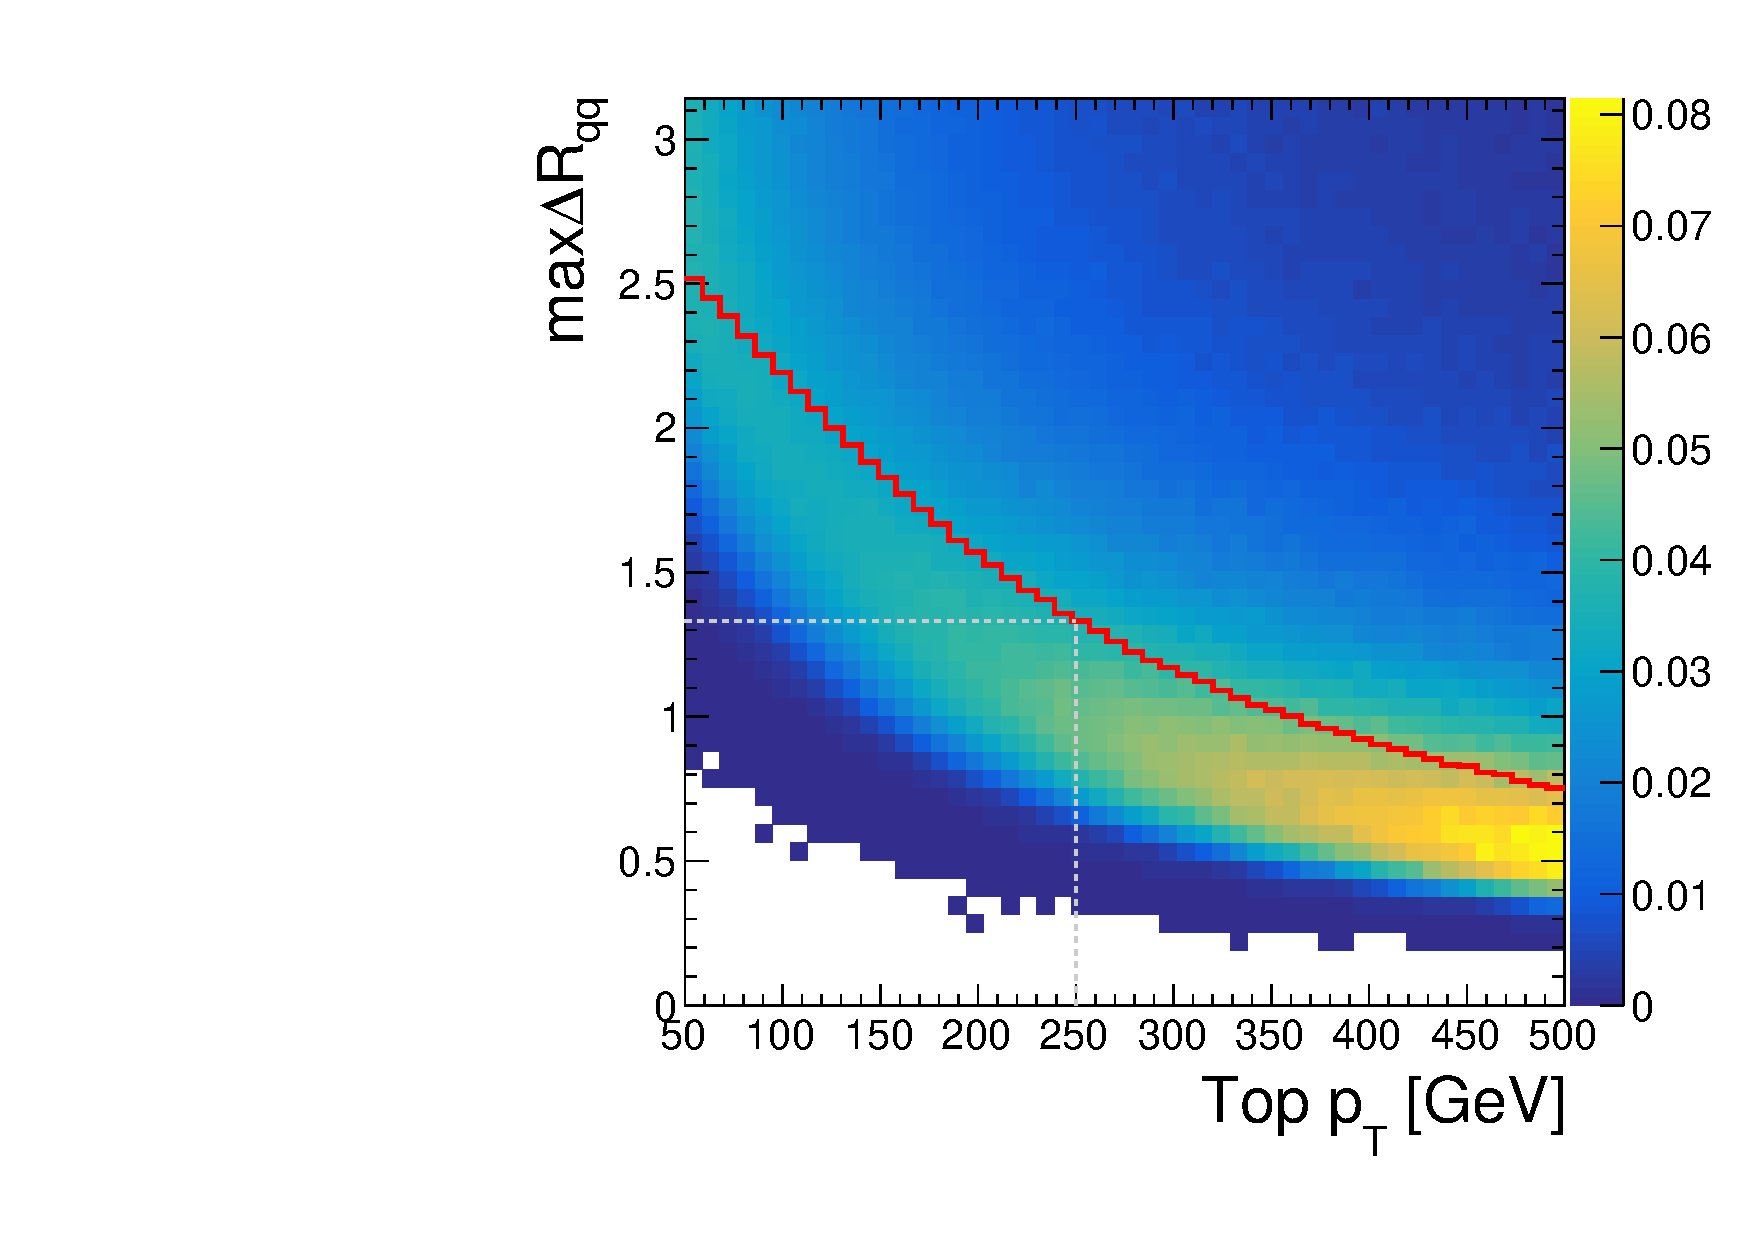
\includegraphics[width=0.75\textwidth]{figures/toptagging/gen/ptdr.pdf}
        \caption{Distribution of top quark momenta versus decay radii in a simulated top quark pair sample.
                 The events are weighted such that the inclusive momentum distribution is uniform. 
                 The $z$-axis units are arbitrary, but proportional to the distribution of jets. 
                 The solid red line marks the 50\% quantile of jets at each value of $\pt$. }
        \label{fig:jets:dr}
    \end{center}
\end{figure}

\section{Identification}

\subsection{Substructure}

\subsubsection{A combined tagger}
\label{sec:jets:combined}

\subsection{Heavy flavor identification}

\section{Data validation}
